% !TEX root = ../literature.tex
\subsection{Discussion}
\todo[inline]{Rewrite from scratch.}
%this section needs to be called discussion, and you need to use it to discuss a bit more about the relationships between the different fields, concluding with the idea that some sharing of information across these areas to futher research various aspects would be a good idea. So you are on the right track - but you need to be a bit more detailed in your thinking
\todo{interaction with large displays or just large display?}
This current paper aims to analytically summarize published research within the areas of interaction with large displays, natural user interaction, and cross device interaction.\\. In the current section we would expand on the relationships between presented different fields, we believe this will further deepen our understanding of them.\\
%The findings of this work are that gesture recogntion using touchscreens is now a mature enough technology that it is ready for implementation in commerical products. The iPhone has shown that basic gesturing has a place in mobile operating systems and my results show that more complex gestures can be easily recognised and recognised accurately. The problem is context.
By making the objects that surround us change their non-interactive state to a responsive medium, Buxton and Welnner achieved a novelty supporting Weiser's vision of ubiquitous computing. A secondary objective of Weiser was related to the size of the object. An example of this principle can be related to the work of Cerwinski that shows how size can correlate to the performance in a work environment.
A new state is often related to not only a technologically progress but also conceptual ideas. A Technological example would be the development of the Kinect that provide new interaction possibilities, and a conceptual example is extending the traditional interactive model of a large display by controlling it with a another device (CDI)
\todo[inline]{A new state is often related to not only a technologically progress but also conceptual ideas. A Technological example would be the development of the Kinect that provide new interaction possibilities, and a conceptual example is to use tangible objects as a medium for interacting with the virtual/digital world (rikimoto and kefee)}
This change provides new opportunities and challenges for developing interaction techniques in the interaction space of NUI and CDI. These two identified areas differ in-between, however they also have common ground, we present this idea in \Cref{fig:litreview}.
\todo[inline]{old below}
Many researchers (Buxton and Czerwinski ) had spent time and effort to explore how large displays aid in improving people's experiences. 
With the shift from private to public settings the explored solutions changed. \todo{Is this a good way to say it?}
It was highly impractical to put wires on people who wanted to use an installation naturally in a public environment [9].(Henrik 2013)\\

With this limitation came different approaches for solving it. 
We identified two different areas which deals with it, we present them in \Cref{fig:litreview}. \todo{It isn't really making sense, Before we start mentioning the public space, and now we identify it- wrong order. If it is nui and CDI its probably better to rephrase it all.}

\begin{figure}[h!]
\centering
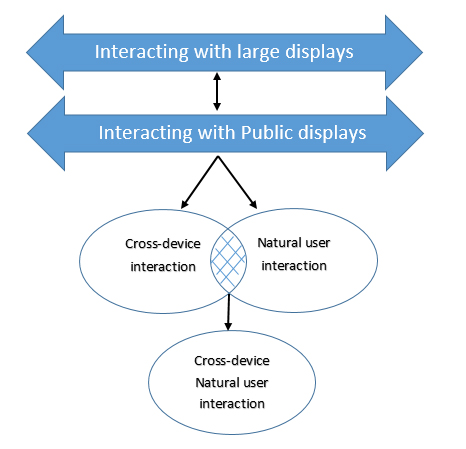
\epsfig{file=images/litreview-fig1.jpg, width=0.5\textwidth}
\caption{Write Caption}
\label{fig:litreview}
\end{figure}
\todo[inline]{Assuming the numbers are right, then keep this. But for god sake, use cite!}
The fields of natural user interactions and cross-device interactions were examined. 
We were surprised to see that research in combining features from the two areas is slim even though they are complementary to each other. 
There was research that was done [26, 27, 28, 29]. 
Interaction-techniques were evaluated with 3-6 people using qualitative surveys in [27,28,29] and without qualitative surveys in [26].\\

In summary, we can see research opportunities in further exploration of cross-device natural user interactions technique for large displays. We believe the limitations that each of these fields ignore is the interaction space between them. To move beyond this limitation, we believe a unification of these discrete interaction techniques in continuous interaction space and it's further research would be positive and beneficial.
Firstly, as handheld devices become thinner and lighter and spatially-aware technologies, such as Kinect, continue to evolve, this opens a potentially rich space of aforementioned techniques. 
Secondly, we see opportunities in quantitative aspect, for example comparative study of different interaction techniques. 
